\documentclass[tikz,border=2mm]{standalone}

\usepackage{bm}
\usepackage{xcolor}
\usetikzlibrary{arrows,positioning}
\usetikzlibrary{arrows.meta}

\begin{document}

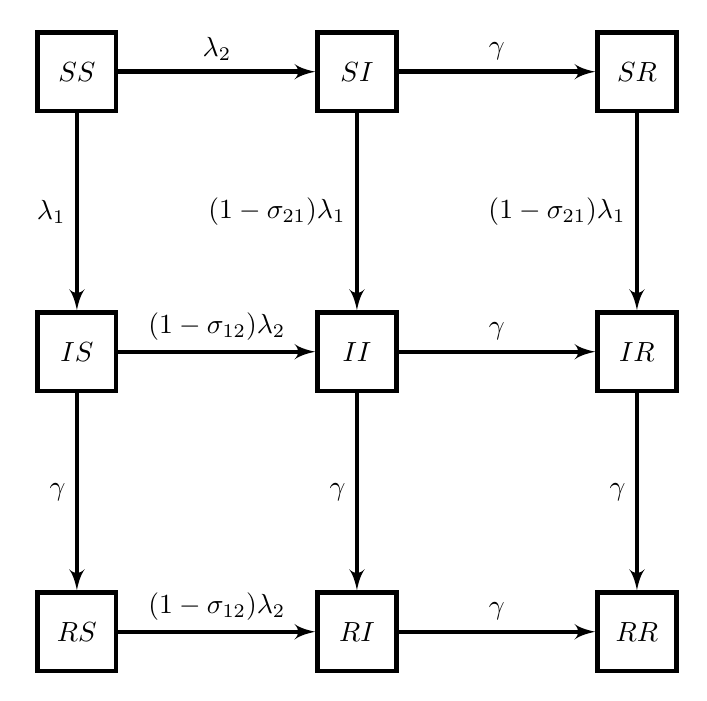
\begin{tikzpicture}[node distance=2.5cm,auto,>=latex',every node/.append style={align=center},int/.style={draw, minimum size=1cm},inverter/.style={rectangle,draw,inner sep=2pt,minimum size=6mm},posnode/.style={shape=rectangle, draw=orange, line width=2},
  negnode/.style={shape=rectangle, draw=black, line width=2}]
    \node [int, ultra thick] (SS)             {$SS$};
    \node [int, below=of SS, ultra thick] (IS)             {$IS$};
    \node [int, below=of IS, ultra thick] (RS)             {$RS$};
    \node [int, right=of IS, ultra thick] (II)             {$II$};
    \node [int, right=of II, ultra thick] (IR)             {$IR$};
    \node [int, right=of SS, ultra thick] (SI)             {$SI$};
    \node [int, right=of SI, ultra thick] (SR)             {$SR$};
    \node [int, right=of RS, ultra thick] (RI)             {$RI$};
    \node [int, right=of RI, ultra thick] (RR)             {$RR$};
    \path[->, ultra thick, left] (SS) edge node {$\lambda_1$} (IS);
    \path[->, ultra thick, left] (IS) edge node {$\gamma$} (RS);
    \path[->, ultra thick, left] (IR) edge node {$\gamma$} (RR);
    \path[->, ultra thick, above] (SS) edge node {$\lambda_2$} (SI);
    \path[->, ultra thick, above] (SI) edge node {$\gamma$} (SR);
    \path[->, ultra thick, above] (RI) edge node {$\gamma$} (RR);
    \path[->, ultra thick, above] (RS) edge node {$(1-\sigma_{12}) \lambda_2$} (RI);
    \path[->, ultra thick, left] (SR) edge node {$(1-\sigma_{21}) \lambda_1$} (IR);
    \path[->, ultra thick, above] (IS) edge node {$(1-\sigma_{12}) \lambda_2$} (II);
    \path[->, ultra thick, left] (SI) edge node {$(1-\sigma_{21}) \lambda_1$} (II);
    \path[->, ultra thick, left] (II) edge node {$\gamma$} (RI);
    \path[->, ultra thick, above] (II) edge node {$\gamma$} (IR);
\end{tikzpicture}
\end{document}
